\chapter{Metodologia}
\section{Processo de construção de uma aplicação de Aprendizado de Máquina}

Segundo o guia do desenvolvedor de aprendizado de máquina da \cite{Amazon} e o livro \textit{Hands-on machine learning with Scikit-Learn and TensorFlow: concepts, tools, and techniques to build intelligent systems} escrito por \cite{geron2017hands}, o processo de desenvolvimento de uma aplicação de aprendizado de máquina é iterativo e envolve uma série sequencial de passos que de maneira geral vão desde entender a \textit{big picture} até a apresentação da solução de proposta da aplicação. O processo pode ser visualizado pela representação \textit{Business Process Model and Notation} - BPNM - da figura:

Figura do processo \citeonline{geron2017hands}

\subsection{Abstrair o problema no contexto}
O primeiro passo é entender o que é será predito, ou seja analisar a natureza do problema observando quais respostas o modelo escolhido deverá predizer, para auxiliar na solução do problema \cite{geron2017hands}.

Imagine o seguinte cenário, no qual você deseja fabricar produtos, porém sua decisão de qual produto fabricar depende do número de vendas em potencial. Nesse cenário, você precisa saber a quantidade de vezes que cada produto foi comprado, ou seja, predizer o número de vendas. Existem diversas maneiras de definir esse problema utilizando AM, porém a escolha  zde como definir o problema depende do seu caso de uso ou necessidade comercial \cite{Amazon}.

Em termos mais técnicos dentro do AM, o ponto importante do entendimento do contexto e a abstração do problema, é que essa etapa tem um papel fundamental na escolha dos modelos, pois tendo o entendimento da natureza do problema será selecionado o modelo para predizer os resultados para esse dado problema com base no tipo de aprendizado mais adequado a este contexto.

Além disto é necessário definir claramente quais os objetivos deverão ser atingidos, qual a métrica de desempenho utilizar para validar o modelo, quais algoritmos utilizar, qual o desempenho esperado e com estas e outras respostas será possível enquadrar o problema, é supervisionado, não supervisionado ou por reforço? É classificação, regressão ou outra coisa\cite{geron2017hands}. Enfim essa etapa de análise serve para orientar o trabalho para evitar a criação de modelos que não respondem o problema além de otimizar o esforço no desenvolvimento \cite{Amazon}.

\subsection{Coleta de dados}

Os dados coletados nessa etapa devem estar ligado diretamente ao que é requerido pelo problema e atender esses requisitos a fim de atender as necessidades do contexto é de suma importância, pois alguns dos já citados desafios encontrados no desenvolvimento de sistema de AM estão relacionados aos dados que serão utilizados \cite{geron2017hands}

A quantidade de dados coletados nessa etapa ainda é incerta, porém é levado em consideração que quanto maior a quantidade de dados coletados, melhor. A quantidade de dados coletados nessa etapa ainda é incerta, porém é levado em consideração que quanto maior a quantidade de dados coletados, melhor. Neste trabalho é utilizado sinais neuromusculares captados por dispositivos sEMG. 

\subsection{Analisar os Dados}

Antes de passar os dados para o algoritmo de AM é considerado uma boa prática inspecionar seus dados para identificar problemas e obter \textit{insights} sobre os dados que se está utilizando \cite{Amazon}, quanto melhor for os dados, melhor será o modelo preditivo que está utilizando esses dados.

Segundo o guia do desenvolvedor de aprendizado de máquina da Amazon, enquanto você está analisando seus dados é importante responder às seguintes perguntas:
\begin{itemize}  
    \item Os dados correspondem às suas expectativas?
    \item Houveram problemas nas coletas dos dados?
    \item Quais classes são as mais frequentes dentre os seus dados?
    \item Existem mais valores ausentes ou inválidos do que o esperado?
\end{itemize}

Além de construir um resumo dos dados relacionados a essas perguntas, também é uma boa prática conhecer a correlação entre cada variável e a classe de destino. Em geral, você deseja incluir variáveis com alta correlação, porque elas são aquelas com maior poder preditivo (sinal) e deixam de fora as variáveis com baixa correlação, porque são provavelmente irrelevante \cite{Amazon}. 

Essas práticas são importantes para conhecer os dados que serão utilizados podendo prevenir ou facilitar a identificação de possíveis erros futuros com relação a utilização dos dados.

\subsection{Processar Dados}

Após a etapa de análise dos dados, é necessário tornar as variáveis mais significativas. essa etapa é conhecida como processamento de \textit{features}, sendo responsável por preparar os dados para serem consumidos pelos algoritmos de AM e consiste em três etapas mais comuns \cite{prepareDataML}..

\begin{enumerate}
    \item \textbf{Formatar}: Os dados selecionados podem não estar no formato desejado ou os dados estão em um banco de dados relacional e é desejado que os mesmos estejam em um arquivo simples. Formatar os dados para um padrão que facilita o trabalho com esses dados é a primeira etapa do processamento.
    \item \textbf{Limpar}: Remover ou consertar os dados que faltam dentro de um banco de dados  Pode haver instâncias de dados incompletas e não conter os dados que você acredita que precisam solucionar o problema. Essas instâncias podem precisar ser removidas. Além disso, pode haver informações confidenciais em alguns dos atributos e esses atributos podem precisar ser anonimizados ou removidos dos dados completamente.
    \item \textbf{Selecionar Amostras}: No caso de se trabalhar com uma grande massa de dados, nem sempre todos esses dados serão utilizados. A quantidade exagerada de dados pode levar à tempos de execução muito elevados e maiores requisitos computacionais. Selecionar uma amostra representativa dos dados selecionados pode ser muito mais rápida para explorar os resultados.
\end{enumerate}

\subsection{Selecionar o Modelo}
Após identificar o problema, explorar os dados, testar e limpar as incoerências e prepara os dados além de separa os dados em treino e teste, agora é possível escolher o modelo adequado para solucionar o problema identificado \cite{geron2017hands}.

\subsection{Treinar o Modelo}
Agora para Treinar o modelo, com os a totalidade do dados separados em por exemplo 80\% dados de treino e 20\% em dados de teste, utilizar os 80\% dos dados para treinar o modelo, passando estes dados pelo algoritmo escolhido, os outros 20\% restantes serão utilizados para testar a eficiência da rede. 

\subsection{Validar a solução}
Para validar a solução, pode-se utilizar a matriz de confusão \ref{matriz_consusao} bastante utilizada em AM para visualizar o comportamento de modelos em classificação supervisionada, basicamente separa-se os dados em uma matriz com valores previstos e valores verdadeiros, cruza-se estes dados em positivos e negativos \cite{caelen2017bayesian}.

\begin{figure}[!htb]
	\centering
	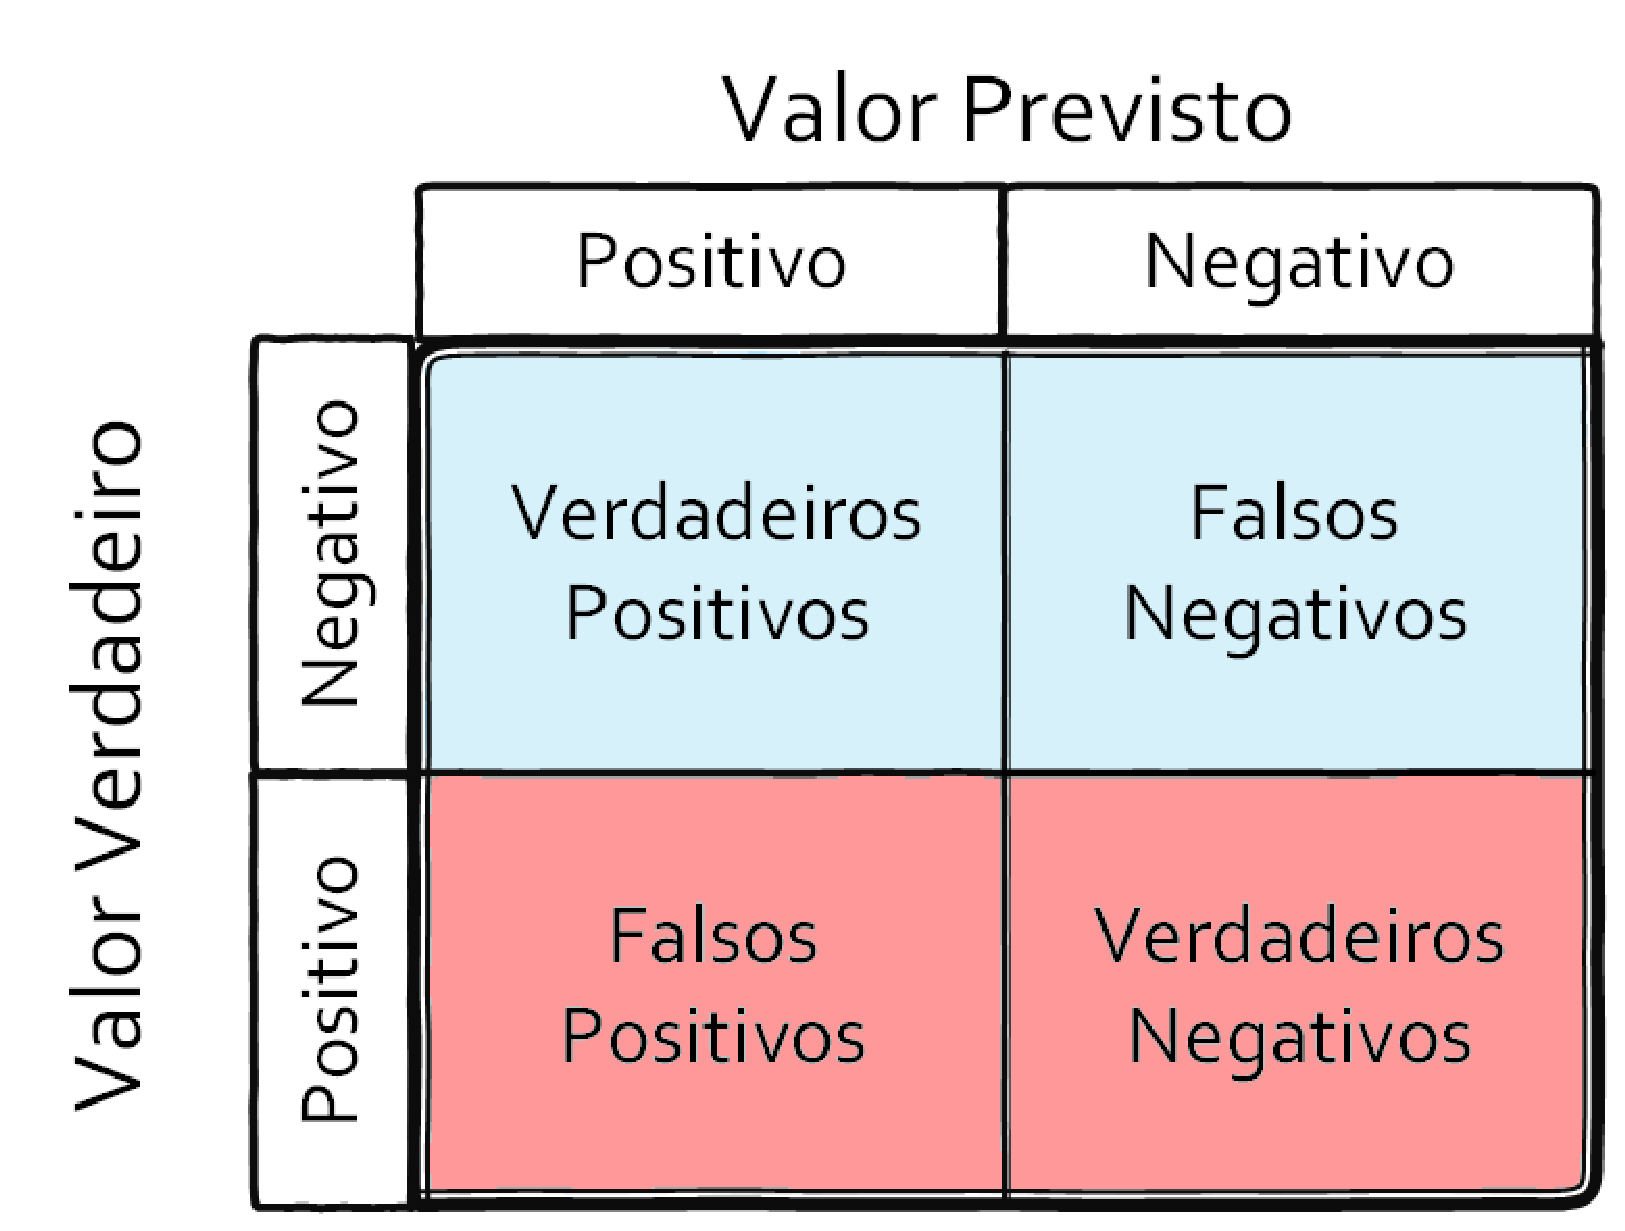
\includegraphics[width=0.8\textwidth]{figuras/matriz_consusao.eps}
	\caption{Exemplificação da matriz de confusão, adaptado de \citeonline{AndreoniMartin}}
	\label{matriz_consusao}
\end{figure}

\subsection{Apresentar a solução}
Construir visualizações informativas é uma das mais importantes tarefas dentro da análise de dados \cite{McKinney2012datapython}. Essa etapa consiste na utilização de ferramentas e técnicas para a representação dos dados obtidos tanto pelo modelo quanto pelos dados coletados, para validação dos mesmos. O resultados obtidos pelo algoritmo de AM sobre os dados de coleta serão aferidos quanto ao seu \textit{benchmarking} \cite{Benchmarking} para avaliar o seu desempenho, análise de acurácia e precisão como também para avaliar seu tempo de resposta. A apresentação dos dados da coleta tem por objetivo avaliar tanto a separação do espaço amostral dos dados quanto para se obter um comparativo que melhor represente de maneira visual os dados após a filtragem da etapa do processamento dos dados, de maneira geral serve para ajudar a identificar \textit{outliers} ou transformações de dados necessárias, ou como uma forma de gerar ideias para modelos \cite{McKinney2012datapython}.	
	
A tecnologia utilizada para o desenvolvimento neste trabalho, python, possui muitas bibliotecas complementares para fazer visualizações estáticas ou dinâmicas, mas focaremos principalmente no matplotlib e nas bibliotecas criadas com base nele \cite{McKinney2012datapython}, por se tratar de uma ferramenta versátil e ser a que mais foi citada dentro de pesquisas sobre visualização de dados com Python.

O Matplotlib é uma biblioteca de plotagem 2D em Python que produz números de qualidade de publicação em uma variedade de formatos impressos e ambientes interativos entre plataformas. O Matplotlib pode ser usado em scripts Python, nos shells do Python e do IPython, no notebook Jupyter, nos servidores de aplicativos da Web e em quatro kits de ferramentas de interface gráfica do usuário \cite{Matplotlib}.
